% This is a template file for submitting your homework in math 301. 

\documentclass[letter]{article} %This tells the LaTeX compiler what type of document we are creating

%The next few lines are packages that we load. Geometry allows us to change the margins and other page properties. The amsmath and amssymb packages give us access to common math symbols. 

\usepackage[margin=1in]{geometry}
\usepackage{amsmath}
\usepackage{amssymb}
\usepackage{ifthen}
\usepackage{fancyhdr}
\usepackage{color}
\usepackage[fleqn]{nccmath}
\usepackage{graphicx}
\usepackage{hyperref}
%\graphicspath{ {C:/Users/joh10/Desktop/FSU/CompStat1/Assignments/hw6/} }

%I would like to have space to write comments on your work.  The linespread command below will add extra space to your document.
\linespread{1.5}
 
\pagestyle{fancy}
\rhead{\ifthenelse{\value{page}=1}{\noindent Homework 7 - FSA for Multi-Class Data \hfill Kyle Shaw, Thomas Johansen \\
Oct. 27, 2017 \hfill STA 5635}{Shaw/Johansen}}

\rfoot{\thepage}
\renewcommand{\headrulewidth}{0pt}
\renewcommand{\footrulewidth}{0pt}
\cfoot{}

%We are now ready to start our document.  The next line tells the computer to start creating the PDF. 
\begin{document}
\setlength{\headsep}{0.5 in}
%The section* command below creates an unnumbered section.  If you remove the *, you'll see it numbers the section as section 1. 

\section*{Satimage}

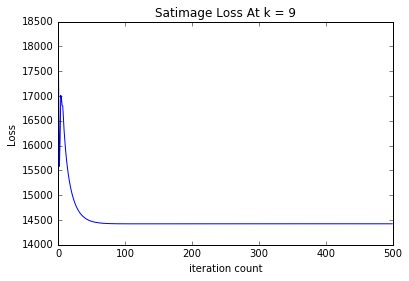
\includegraphics[scale=1]{sat_loss} \\
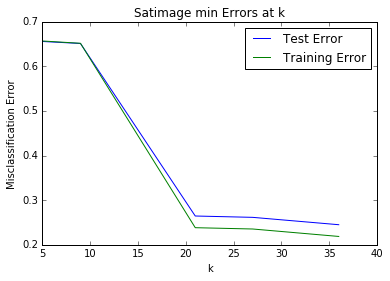
\includegraphics[scale=1]{sat_err}


\section*{Cov-Type}

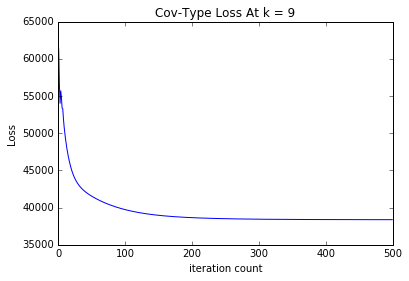
\includegraphics[scale=1]{cov_loss} \\
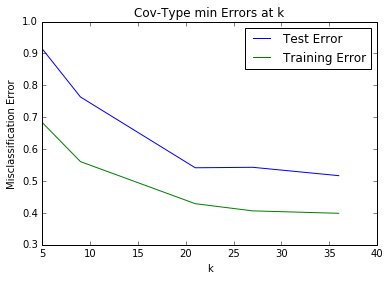
\includegraphics[scale=1]{cov_err}


\section*{Misclassification Error}

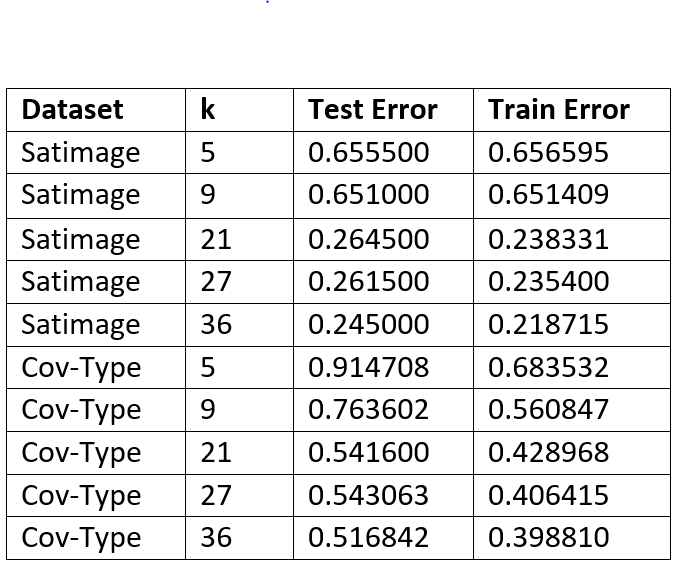
\includegraphics[scale=1]{table}


\section*{Code}

Included are functions for training and updating the weights, and setting the schedule for eliminating variables. For full code see \url{https://github.com/johansent/ML_Fall2017/tree/master/hw7}.

\begin{verbatim}
def updateWeights1(X,Y,w, Ncol,Nrow, learningRate, s):
    L = len(w)
    derivative = np.array([[0.0]*(Ncol)]*L)
    lorenz = 0.0
    X = np.array(X)
    U = np.dot(X, np.transpose(w))
    Uy = [U[i][Y[i]] for i in range(Nrow)]
    for l in range(L):
        diff = (Uy - U[:,l]) - 1
        diff = np.array([-((2 * d) / (1 + d*d)) if d <= 0 else 0 for d in diff])
        logical = [l != Y[i] for i in range(Nrow)]
        diff = diff * logical
        lorenz += sum(np.log(1 + diff**2))
        dmat = diff * X.transpose()
        derivative[l] = np.sum(dmat, axis = 1)
    total = [X[i][0] if logical[i] else 0 for i in range(Nrow)] 
    w = w - (learningRate * (derivative + (s * w))) 
    loss = (lorenz + s * np.linalg.norm(w, 'fro'))
    return w, loss

def TrainWeights(X,Y,Xtest,Ytest,niter,k, learnRate = .01):
    Nrow = len(X)
    Ncol = len(X.columns)
    L = 7
    X1 = X.copy()
    Xtest1 = Xtest.copy()
    s = .001    
    w = np.array([[0]*(Ncol)]*L)    
    loss = []
    testErrors = []
    trainingErrors = []
    for i in range(niter): 
        w, newloss = updateWeights1(X1,Y,w, Ncol,Nrow, learnRate, s)
        loss.append(newloss)
        if Ncol > k:
            Mi = getMi(Ncol, k, niter, i, u = 100)
            w,X,Xtest,Ncol = getMBest(w, X1, Xtest1, Mi, Ncol)
        testErrors.append(Test(w,Xtest1, Ytest))
        trainingErrors.append(Test(w,X1,Y))
        if(i % 50 == 0):
            print('i', i)
    return testErrors,trainingErrors, loss

def getMi(M, k, N, i, u = 100):
    return round(k + (M - k) * max([0,(N - 2 * i)/(2 * i * u + N)]))
    
def getMBest(w, X, Xtest, M, Ncol):
    summation = sum(w)
    best = sorted(range(len(summation)), key=lambda i: summation[i])[-M:]
    worst = sorted(range(len(summation)), key = lambda i: summation[i])[0:(Ncol - M)]
    w = np.array([[x[i] for i in sorted(best)] for x in w])
    X.drop(X.columns[worst], axis=1, inplace=True)
    Xtest.drop(Xtest.columns[worst], axis=1, inplace=True)
    return w, X, Xtest, len(X.columns)
\end{verbatim}

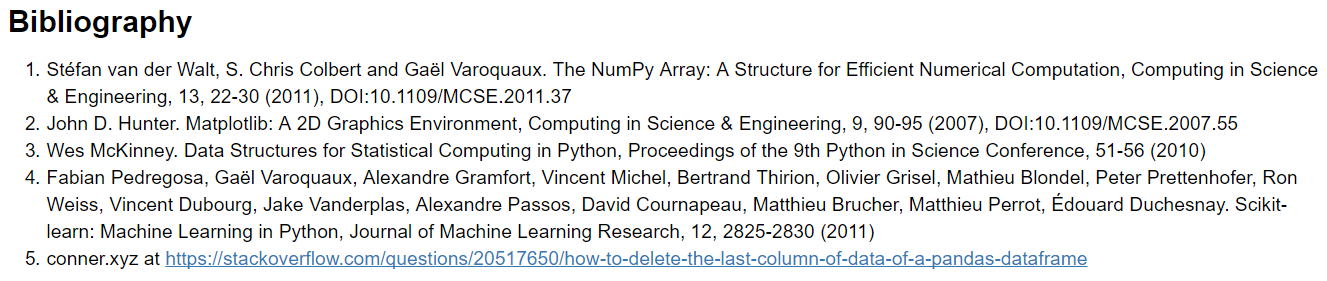
\includegraphics[scale=0.6]{bib}



%\clearpage
%\newgeometry{top=1in, bottom=1in, left=0.5in}


\end{document}














